\documentclass{standalone}
\usepackage{tikz}
\usepackage{xcolor}

\usetikzlibrary{decorations.pathmorphing}
\usetikzlibrary{shapes}
\usetikzlibrary{shapes.geometric}

\begin{document}
	
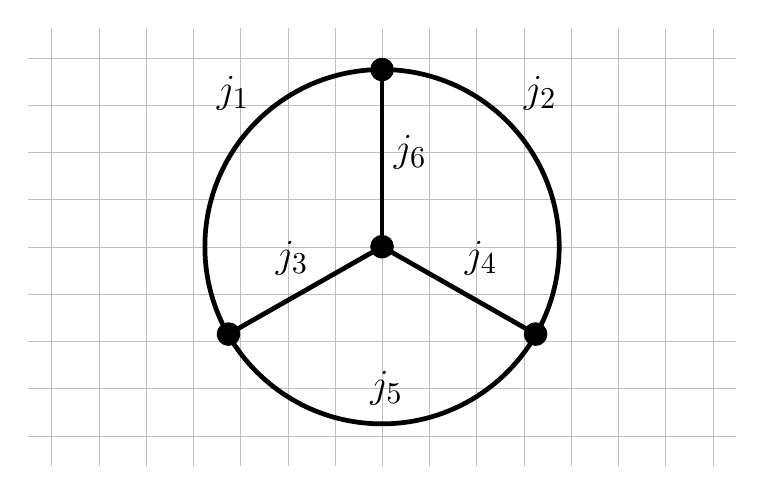
\begin{tikzpicture}[ thick,scale=3]
	
	% (VP_ml-B)
	\draw[gray!50,line width=0.01mm,step=0.2] (-0.5,0.073) grid (2.5, 1.927);
	\draw[line width=0.6mm] (1,1) circle (.75);
\fill (1,1.75) circle (0.05);
\fill (0.35,0.63) circle (0.05);
\fill (1.65,0.63) circle (0.05);
\fill (1,1) circle (0.05);
\draw[line width=0.6mm] (1, 1) -- (1, 1.75);
\draw[line width=0.6mm] (1, 1) -- (0.35, 0.63);
\draw[line width=0.6mm] (1, 1) -- (1.65, 0.63);
	\node at (0.35,1.65) {\fontsize{15pt}{0} $j_1$};
	\node at (1.65,1.65) {\fontsize{15pt}{0} $j_2$};
	\node at (0.6,0.95) {\fontsize{15pt}{0} $j_3$};
	\node at (1.4,0.95) {\fontsize{15pt}{0} $j_4$};
	\node at (1,0.4) {\fontsize{15pt}{0} $j_5$};
	\node at (1.1,1.4) {\fontsize{15pt}{0} $j_6$};


\end{tikzpicture}

\end{document}